\documentclass[a4paper]{article}
\usepackage[left=3cm,right=3cm,top=2cm,bottom=2cm]{geometry} % page settings
\usepackage{enumerate}
\usepackage{hyperref}
\usepackage{graphicx}
\usepackage{amsfonts}
\usepackage{amsthm}
\usepackage{mathtools}
\usepackage{titlesec}
\usepackage{polski}
\usepackage{tikz}
\usepackage[utf8]{inputenc}
\DeclarePairedDelimiter\ceil{\lceil}{\rceil}
\DeclarePairedDelimiter\floor{\lfloor}{\rfloor}
\DeclarePairedDelimiter\set{\lbrace}{\rbrace}


\def\checkmark{\tikz\fill[scale=0.3](0,.35) -- (.25,0) -- (1,.7) -- (.25,.15) -- cycle;} 

\titlespacing*{\subsection}
{0ex}{10ex}{3ex}

\title{Lista 4}
\author{Kamil Matuszewski}
\date{\today}

\begin{document}

\maketitle
\setlength{\parindent}{0.5ex}
\setlength{\parskip}{1.5ex}
\newcommand{\R}{\mathbb{R}}
\newcommand{\N}{\mathbb{N}}


\begin{center}
\begin{tabular}{|c *{8}{|c} |c|}\hline
1 & 2 & 3 & 4 & 5 & 6 & 7 & 8 & 9 & 10\\
\hline 
 &\checkmark &\checkmark &\checkmark &\checkmark &\checkmark & & & &\\
\hline
\end{tabular}\\
\end{center}

\subsection*{Zadanie 2}
Ułóż algorytm który dla danego $n$-wierzchołkowego drzewa i liczby $k$ pokoloruje jak najwięcej wierzchołków tak, by na każdej ścieżce prostej było nie więcej niż $k$ wierzchołków pokolorowanych.

Dla każdego wierzchołka ustalimy warstwę. Warstwy naszego drzewa będą wyglądać następująco: w warstwie $i$ będą wszystkie liście powstałe po usunięciu wierzchołków z poprzednich warstw.\\
Teraz, dla danego $k$, jeśli $k$ jest parzyste, to zaznaczamy wszystkie wierzchołki z pierwszych $\frac{k}{2}$ warstw. Jeśli $k$ jest nieparzyste, to dodatkowo bierzemy dowolny niepomalowany wierzchołek.\\
Wszystko to można zrealizować np trzymając kolejkę wierzchołków o stopniu 1. Usuwając kolejne warstwy aktualizujemy stopnie wierzchołków.
Algorytm może wyglądać jakoś tak:
\\ \\
warstwa=1;\\
Dopóki istnieją jakieś wierzchołki:\\
\hspace*{2ex}Dla każdego liścia $v$, włóż $v$ do kolejki.\\
\hspace*{2ex}Dla każdego $v$ z kolejki, jeśli $warstwa\leq \frac{k}{2}$ pomaluj v. Usuń v z grafu (pomocniczego?).\\
\hspace*{2ex} warstwa++\\
Jeśli $k$ $mod$ $2$ $==$ $1$ pomaluj dowolny niepomalowany wierzchołek (o ile istnieje);



$Lemat\ 1:$ Algorytm jest optymalny.
\begin{proof}
Pseudodowód:
Weźmy rozwiązanie optymalne. Sprowadźmy je do naszego. Więcej wierzchołków w naszym rozwiązaniu pomalować się nie da, bo istniałaby ścieżka, w której jest więcej niż k wierzchołków pomalowanych. Dlatego rozwiązanie optymalne musi nie malować wszystkich wierzchołków z naszych $\frac{k}{2}$ warstw, w zamian malując inne. Weźmy wierzchołek z $\frac{k}{2}$ warstw który jest niepomalowany w rozwiązaniu optymalnym - dokładniej weźmy dowolny wierzchołek z najniższej możliwej warstwy. Tą warstwę nazwiemy $l$, wierzchołek $v$. Weźmy pomalowany w rozwiązaniu optymalnym wierzchołek, taki, że leży on powyżej warstwy $l$ i pomiędzy nim a $v$ nie ma żadnych wierzchołków. To, że taki istnieje jest oczywiste, bo $l\leq \frac{k}{2}$, oraz, jeśli by takiego nie było, to rozwiązanie optymalne byłoby mniej liczne niż nasze. Ten wierzchołek nazwiemy $w$. Sprawdźmy, że możemy pomalować $v$ kosztem $w$ nie psując naszego pokolorowania tj na dowolnej ścieżce będzie nie więcej niż k pomalowanych wierzchołków. Weźmy dowolną ścieżkę. Mamy sytuacje:
\begin{itemize}
\item Ścieżka nie zawiera $v$ oraz $w$ - zmiana pokolorowania w tym przypadku nic nie zmienia.
\item Ścieżka zawiera $v$ oraz $w$  - znów, zmiana pokolorowania nic nam nie zmienia.
\item Ścieżka zawiera $w$, nie zawiera $v$ - "odmalowanie" $w$ i pomalowanie $v$ zmniejszy nam liczbę pomalowanych wierzchołków na tej ścieżce, więc z pewnością nic się nie popsuje.
\clearpage
\item Ścieżka zawiera $v$ nie zawiera $w$.\\
Tu sprawa się lekko komplikuje. Oznaczmy ścieżkę $x$ $x'$ naszą rozpatrywaną ścieżką, ścieżkę $x$ $y$ ścieżką zawierającą zarówno $v$ i $w$, a $u$ jako wierzchołek, leżący pomiędzy $v$ i $w$ który rozdziela te dwie ścieżki (musi taki istnieć). Rozpatrzmy rozwiązanie optymalne. Na ścieżce $u$ do $y$ poza $w$ było przynajmniej $l-1$ wierzchołków pomalowanych, jako, że $l$ była najmniejszą warstwą z niepomalowanym wierzchołkiem. Do tego dochodzi $w$, mamy więc przynajmniej $l$ wierzchołków pomalowanych na tej ścieżce. Na ścieżce $u$ do $x'$ nie może być więc więcej niż $k-l$ wierzchołków pomalowanych, bo w rozwiązaniu optymalnym na ścieżce $x'$ do $y$ nie mogło być więcej niż $k$ wierzchołków pomalowanych. Teraz, dla ścieżki $x$ do $u$ mamy dokładnie $l-1$ wierzchołków pomalowanych - ponownie, przynajmniej $l-1$, a do tego pomiędzy $v$ a $w$ a w szczególności $v$ a $u$ nie ma wierzchołków pomalowanych. Stąd, na ścieżce $x$ do $x'$ w rozwiązaniu optymalnym mamy maksymalnie $k-l+(l-1)=k-1$ wierzchołków pomalowanych. Dokładając do tego $v$ otrzymujemy $k$ wierzchołków, więc nic się nie psuje. 
\end{itemize}
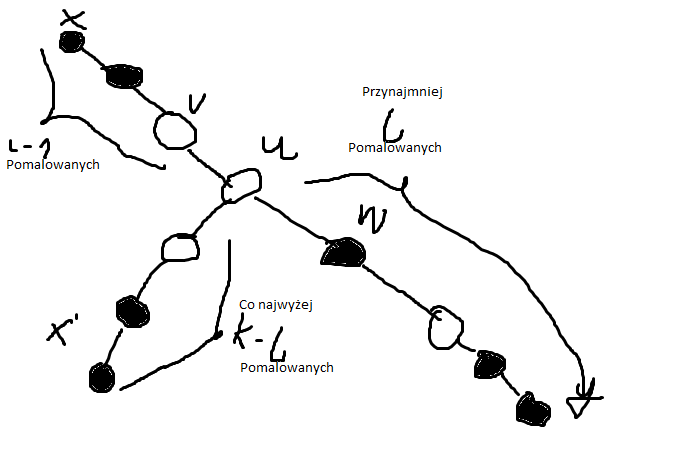
\includegraphics[scale=0.8]{pomocnaukowa.png}

Gdy $k$ jest nieparzyste, odmalujmy dowolny wierzchołek. Mamy parzyste, możemy sprowadzić do rozwiązania optymalnego. Nasz algorytm maluje dowolny wierzchołek, więc sprowadziliśmy rozwiązanie do optymalnego.

Teraz, widać, że dowolne rozwiązanie optymalne można przekształcić tak, by w $\frac{k}{2}$ warstw wszystkie wierzchołki były pomalowane. Skoro nie da się pomalować więcej, to nasze rozwiązanie jest tak dobre jak formalne.
\end{proof}

\subsection*{Zadanie 3}
Mamy n odcinków $I_j=<p_j,k_j>$, leżących na OX. Ułóż algorytm znajdujący zbiór nieprzecinających się odcinków o największej mocy.


Posortujmy odcinki względem $k_j$, tj względem końca odcinka. Bierzmy kolejne odcinki z tak posortowanej listy, o ile początek jest większy-równy końcowi poprzedniego.
\begin{proof}

Mamy uporządkowanie A, załóżmy, że istnieje lepsze uporządkowanie B. Weźmy pierwsze odcinki które się różnią w naszych uporządkowaniach, tj $A_i\neq B_i$. Mamy następujące opcje:
\begin{itemize}
\clearpage
\item $B_i$ kończy się wcześniej niż $A_i$. Wtedy nasz algorytm wybrałby ten odcinek. Skoro go nie wybrał, to $B_i$ kończy się albo w tym samym miejscu albo później niż $A_i$ co jest sprzeczne z założeniem.
\item $B_i$ kończy się w tym samym momencie co $A_i$. Wtedy to czy wybierzemy w tym kroku $B_i$ czy $A_i$ nie ma znaczenia, bo i w jednym i w drugim uporządkowaniu możemy wybrać te same elementy. Sprzeczne z tym, że B jest lepsze od A.
\item $B_i$ kończy się później niż $A_i$. Wtedy uporządkowanie B może być albo tak samo dobre (w sensie tak samo liczne) co A, lub gorsze (w sensie mniej liczne), gdyż kończy się później, i w najlepszym wypadku nie zmniejszy nam liczby możliwych do wybrania odcinków w kolejnym kroku, albo zablokuje nam dostęp do jakiegoś odcinka (odcinek skończy się później niż zacznie się jakiś inny). Sprzeczne z tym, że B lepsze od A.
\end{itemize}

\end{proof}

\subsection*{Zadanie 4}
Dla danych $a\leq b$ chcemy przedstawić $\frac{a}{b}$ jako sumę różnych ułamków o licznikach równych 1. Udowodnij, że algorytm zawsze znajdzie rozwiązanie, oraz, że nie będzie to rozwiązanie optymalne.

$$\frac{x}{y}=\frac{1}{\ceil{y/x}}+\frac{(-y \mod x)}{y\ceil{y/x}}=\frac{y+(-y \mod x)}{y\ceil{y/x}}\stackrel{*}{=}\frac{y+x\ceil{y/x}-y}{y\ceil{y/x}}=\frac{x\ceil{y/x}}{y\ceil{y/x}}=\frac{x}{y}$$

$$*\quad (n \mod k) = n-\floor*{\frac{n}{k}} k\Rightarrow (-n \mod k) = -n-\floor*{\frac{-n}{k}} k = -n-\left(-\ceil*{\frac{n}{k}}\right) k = k\ceil*{\frac{n}{k}} - n $$

Algorytm polega na rozpisywaniu ułamka na sumę dwóch ułamków: jednego o liczniku 1, a drugiego dowolnego. W następnym kroku rozpisujemy ten drugi ułamek (o ile jest taka potrzeba). Proces powtarzamy aż do uzyskania dobrej sumy (tj sumy ułamków o licznikach równych 1).

$Lemat\ 1:$ Algorytm zachłanny zawsze daje rozwiązanie.
\begin{proof}
Zauważmy, że wystarczy sprawdzić, że nasz algorytm się skończy. Otrzymamy dobrą postać, ponieważ zawsze otrzymujemy jeden poprawny ułamek a na drugim ponownie wywołujemy algorytm (jeśli licznik $\geq$ 1). Jeśli algorytm się skończy, będziemy mieli dobrą postać.\\
To, że algorytm się skończy, jest proste do pokazania. Zauważmy, że w dowolnym przypadku, $a \mod x < x$. Dodatkowo, $\mod x$ zawsze zwraca liczbę naturalną. Więc licznik naszego ułamka będzie się zmniejszał o przynajmniej 1. Skoro x jest liczbą naturalną, to po skończonej liczbie kroków $a \mod x = 1$, czyli otrzymamy poprawny ułamek. \\
Ps. Nie wiem co w wypadku jeśli $-y \mod x$ zwróci 0. To chyba trzeba rozpatrzeć osobno, ale to jest proste, bo wtedy otrzymamy ułamek o liczniku 0, czyli równy 0, czyli algorytm i tak się skończy.
\end{proof} 

$Lemat\ 2:$ Algorytm zachłanny nie daje rozwiązania optymalnego.
\begin{proof}
Kontrprzykład: $$\frac{9}{20} = \frac{1}{3}+\frac{1}{9}+\frac{1}{180} = \frac{1}{4}+\frac{1}{5}$$
Pierwsza równość - rozwiązanie zachłanne. Druga równość - rozwiązanie optymalne.
\end{proof}

\subsection*{Zadanie 5}
Udowodnij algorytm Borówki.

\href{https://pl.wikipedia.org/wiki/Algorytm_Bor%C5%AFvki}{Tu można poczytać o borówce}

\begin{proof}

Po pierwsze, pokażmy, że w dowolnym kroku algorytmu nie powstanie nam cykl.\\
Załóżmy, że w którymś kroku algorytmu powstał nam cykl. Oznaczmy ten cykl jako C. Niech $v_1,v_2,\dots,v_l$ będą kolejnymi wierzchołkami na tym cyklu, a $e_1,e_2,\dots,e_l$ kolejnymi krawędziami($e_k$ łączy $v_k$ i $v_{i}$, gdzie $i=k+1$ $mod$ $l$). Wtedy dla $v_1$ algorytm wybrał $e_1$, dla $v_2$ $e_2$ itd. Oznacza to, że ($C(e)$ to waga $e$):
$$C(e_1)>C(e_2)>\dots>C(e_l)>C(e_1)$$
Mamy więc sprzeczność (zauważmy, że wagi są różne, dlatego nierówności są ostre).

Po drugie, dla dowolnego superwierzchołka jest on MST.\\
Pseudoindukcja?

W pierwszym kroku: załóżmy, że nasz superwierzchołek V nie jest MST. Weźmy MST i nazwijmy je T. Wtedy istnieje $e$, takie, że $e\not\in E(T) \wedge e\in E(V)$. Dołóżmy tą krawędź do naszego T. Powstał nam cykl. Skoro tak, to istnieje krawędź $e'$ incydentna do tego samego wierzchołka co $e$. Ale nasz algorytm dla tego wierzchołka wybrał e, więc $C(e)<C(e')$, więc jak wybierzemy $e$ zamiast $e'$ to dostaniemy drzewo o mniejszej wadze co daje sprzeczność z tym, że T to MST.

W kolejnych krokach: Weźmy pierwszy krok w którym nie dostaliśmy MST(zakładając że w każdym poprzednim mieliśmy MST dla dowolnego superwierzchołka). Podobnie, nazwijmy superwierzchołek V, a MST T. Nasz V składa się z jakichś spójnych składowych którymi są superwierzchołki z kroku poprzedniego. Teraz, w V istnieje e którego nie ma w T. e musi łączyć superwierzchołki z poprzedniego kroku, bo gdyby była wewnątrz jakiegoś z tych superwierzchołków, to wtedy ten superwierzchołek nie byłby MST co jest sprzeczne z zał. indukcyjnym. Skoro tak, to stosując argumentację analogiczną do tej wyżej, dochodzimy do sprzeczności.

\end{proof}
\iffalse
Alternatywny dowód - Tymoteusz Kaczorowski:\\

CUT PROPERTY (unikalne wagi!)
Krawędź e należy do MST\\
...wtedy i tylko wtedy, gdy...\\
Istnieje podział zbioru wierzchołków grafu na A i B taki, że spośród wszystkich krawędzi mających jeden koniec w A, a drugi w B, e jest najlżejsza.\\

Dowód $=>$\\
Weźmy MST i usuńmy z niego jakąś krawędź e. Dostajemy dwie spójne składowe - niech to będzie ten podział na A i B.\\
e musi być najlżejsze spośród wszystkich krawędzi pomiędzy A i B, bo gdyby istniała inna, lżejsza (nazwijmy ją Janusz)...\\
Po wstawieniu jej do MST - {e} dostajemy nowe drzewo o mniejszej sumarycznej wadze (w - e + Janusz < w, bo Janusz < e). Sprzeczność, czyli faktycznie e było najlżejszą krawędzią łączącą dla tego podziału.\\

Dowód $<=$\\
Kontrapozycja.\\
Weźmy krawędź z grafu krawędź e, która nie należy do MST. Pokażę, że dla każdego podziału na A i B nie jest ona najlżejszą łączącą A i B.
Wstawienie jej do tego MST poskutkuje powstaniem cyklu.\\
Przypuśćmy teraz, że istnieje podział na A i B, że e jest w nim najlżejszą łączącą. Przynajmniej jedna krawędź tego cyklu (Janusz) inna niż e musi przechodzić między A i B (idąc po ścieżce zaczynającej się w końcu e osadzonym w A przechodzimy do B, a potem musimy jakoś wrócić do A). Możemy ją usunąć otrzymując na powrót drzewo, a ponieważ e jest lżejsze od Janusza, to dostajemy nowe, lżejsze MST, sprzeczność - czyli e nie może być najlżejsze dla żadnego podziału wierzchołków.\\

Dowód Boruvki.\\
W dowolnym kroku algorytmu, gdzie bierzemy superwierzchołek i dokładamy najlżejszą krawędź z niego wychodzącą:\\
Podzielmy wierzchołki grafu na A - wierzchołki należące do tego superwierzchołka, oraz B - całą resztę. Najlżejsza krawędź wychodzaca z superwierzchołka jest najlżejszą krawędzią łączącą zbiory A i B, czyli należy do MST z cut property.

Nie musimy właściwie udowadniać, że nie powstanie cykl - ten dowód korzystąjacy z cut property pokazuje, że każda krawędź dodana przez algorytm jest najlżejszą krawędzią łączącą jakiś podział wierzchołków, więc musi należeć do MST.
\fi
\subsection*{Zadanie 6}
$Lemat(circle$ $property):$  jeśli krawędź e nie jest maksymalna na żadnym cyklu z G, to e należy do jakiegoś MST.

\begin{proof}
Załóżmy, że e nie jest maksymalna na żadnym cyklu z G, i nie należy do MST. Mamy dwie opcje:
\begin{itemize}
\item e nie leży na żadnym cyklu.\\
Wtedy w trywialny sposób e należy do MST, więc sprzeczność.
\item e leży na jakimś cyklu.\\
Weźmy MST i dołóżmy e. Postał nam cykl jako, że e nie należało do MST. Na tym cyklu jest jakaś krawędź maksymalna, nazwijmy ją e'. Jeśli ją zabierzemy dostaniemy MST o mniejszej wadze, jako, że $C(e)<C(e')$
\end{itemize}
\end{proof}

Skoro już to wiemy, to nasz algorytm wygląda tak:\\
Wczytaj krawędź e łączącą wierzchołki v i w. Zapamiętaj jej wagę i usuń ją z grafu. Puść lekko zmodyfikowany DFS/BFS po tym grafie zaczynając od v. Lekko zmodyfikowany tzn: jeśli krawędź po której masz zamiar przejść ma większą wagę niż waga e, nie przechodź po tej krawędzi. Jeśli dotarłeś do w zakończ wypisując nie.
Jeśli nie dotarłeś do w a nie masz już gdzie iść(algorytm się zakończył) wypisz tak.

Teraz czemu to działa. Jeśli nie dotarliśmy z v do w po krawędziach o mniejszej wadze niż e, to znaczy, że albo po usunięciu e graf się rozspójnił - wtedy e musi należeć do MST, albo e nie była maksymalna na żadnym cyklu G (bo gdyby była to byśmy przeszli po każdej krawędzi z tego cyklu, czyli w szczególności dotarlibyśmy do w), co z $lematu$ oznacza, że e należy do jakiegoś MST.

\end{document}
